

\chapter{Turnstiles in Stellarator fields}

The tools introduced in Ch.\ref{ch:tangleandturns} in the case of the \textit{ToyBox} of Ch.\ref{ch:toybox} can be applied equally well to a more general magnetic field of an arbitrary toroidal device. In Stellarators, where both the poloidal and toroidal components of the magnetic field are generated, in equilibrium, by a set of coils and associated currents, the Biot-Savart law can be used to determine the value of the field at any point in space. Therefore, for an existing or hypothetical configuration, the Poincaré map $\pmap$ can be defined and the turnstile fluxes can be calculated, thus allowing to quantify the stochasticity, the degree of chaos, present due to a given island chain.

Concretely, the framework provided by 
\href{https://simsopt.readthedocs.io/en/latest}{\textcolor{blue}{\textit{Simsopt}}} from \citeauthor{medasani_hiddensymmetriessimsopt_2024} is employed to calculate the field. It is a very general and well-structured way of dealing with stellarator configurations. It is intended for stellarator design and optimisation and interacts well with some other plasma-specific codes, such as VMEC or SPEC. Simsopt can be used to calculate the field using Biot-Savart directly for each evaluation or to interpolate the field on a mesh, which greatly speeds up the calculation but is less accurate. It also enables the evaluation of the magnetic vector potential $\textbf{A}$.

The heteroclinic search is the longest part of the turnstile flux calculation process and is conducted using the interpolated $\textbf{B}$. On the other hand, the direct calculation of $\textbf{B}$ is used to more precisely search for X-points and determine the turnstile flux.

\section{QUASR configurations}

The \textit{QUAsi-symmetric Stellarator Repository}, \href{https://quasr.flatironinstitute.org/}{\textcolor{blue}{\textit{QUASR}}}, contains at the moment over 320'000 stellarator configurations and was created/assembled thanks to \cite{andrew_giuliani_quasr_nodate}.

The search of configurations can be tuned by coil length, number of field periods, type of quasi-symmetry and many other settings. The database explores the space of possible Stellarator fields, which is infinite, and catalogues a number of possible outcomes of Stellarator optimisation. 

Three hand-picked configurations with major differences in edge magnetic topology are reviewed in this section. This examination suggests that obtaining turnstile fluxes from edge islands of the hypothetical configurations is a feasible process and their inclusion as a target of optimization for the design of future devices is viable and imminent.

\subsection{Many islands}\label{sec:quars-0229079}

The configuration \href{https://quasr.flatironinstitute.org/model/0229079}{\textcolor{blue}{0229079}} is a $\nfp = 3$ stellarator with 3 coils per field period with many small islands and chaos in the edge. \figref{fig:coils-0229079} shows the full torus view of it with two kinds of coils with different currents runed through them picture in grey and blue. A magnetic surface is also shown (what is the color scheme saying ?).

\begin{figure}[H]
    \centering
    \begin{subfigure}[t]{0.49\textwidth}
        \centering
        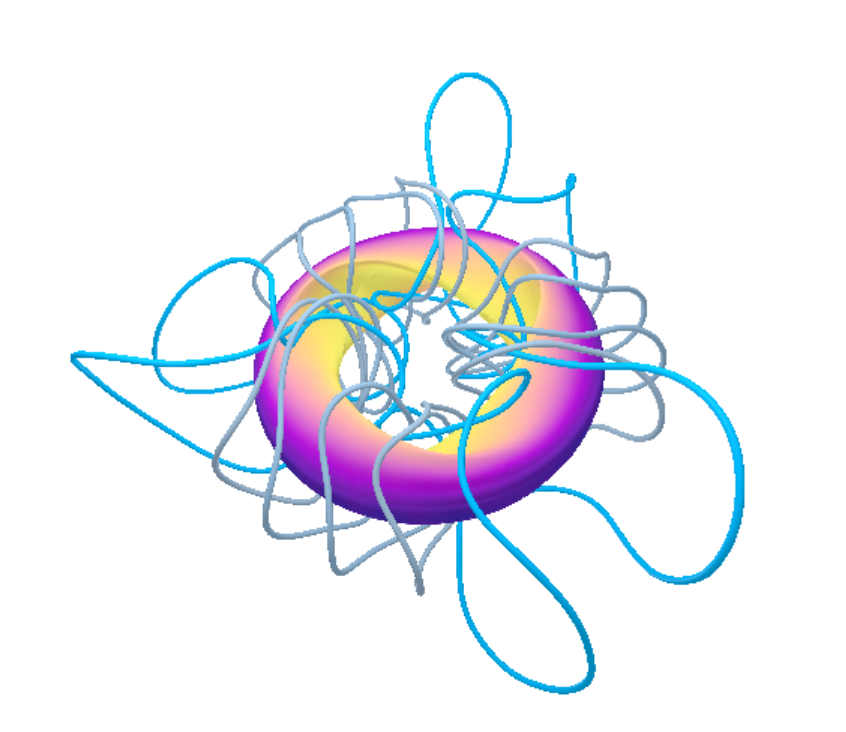
\includegraphics[width=\textwidth]{images/quasrs/config-0229079.png}
        \caption{}
        \label{fig:coils-0229079}
    \end{subfigure}
    \hfill
    \begin{subfigure}[t]{0.49\textwidth}
        \centering
        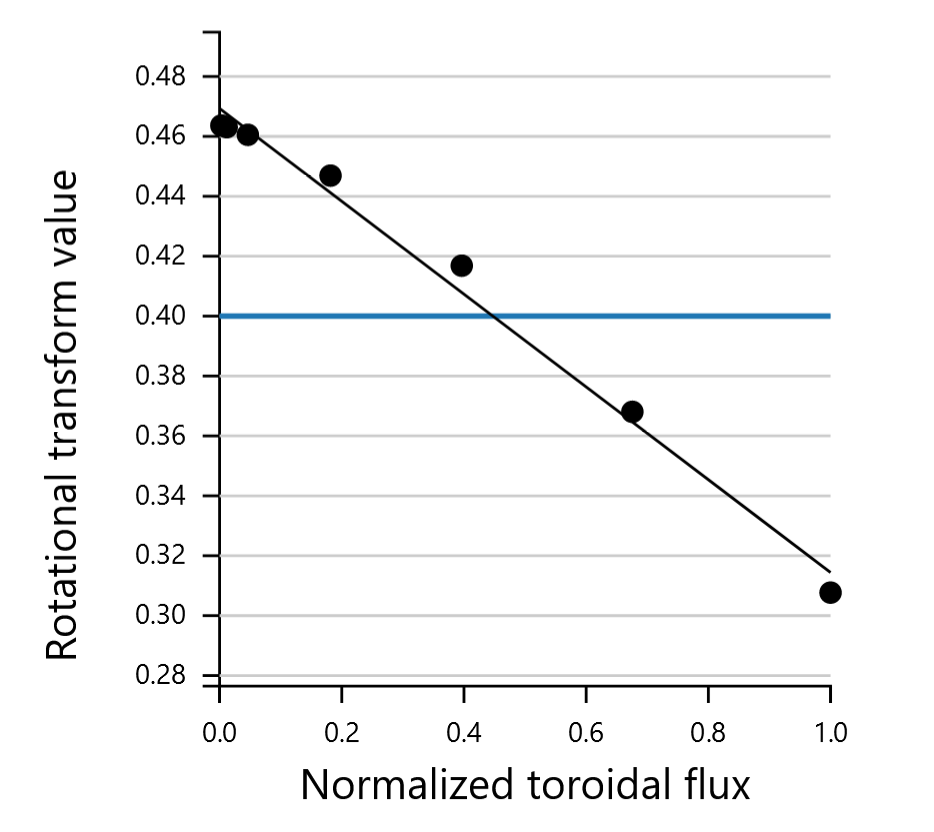
\includegraphics[width=0.8\textwidth]{images/quasrs/iota-0229079.png}
        \caption{}
        \label{fig:iota-0229079}
    \end{subfigure}
    \caption{QUASR configuration 0229079. (a) Coil structure and an external magnetic surface, the same colours indicate the same value of current flowing into the coils. (b) Rotational transform against the normalised toroidal flux and its mean value as a horizontal line.}
    \label{fig:config-0229079}
\end{figure}

The poincare section of such a is shown in \figref{fig:0229079-p} we can see that there are a lot of small islands in the edge. This island is one of the last where the integration is succeeding

\begin{figure}[H]
    \centering
    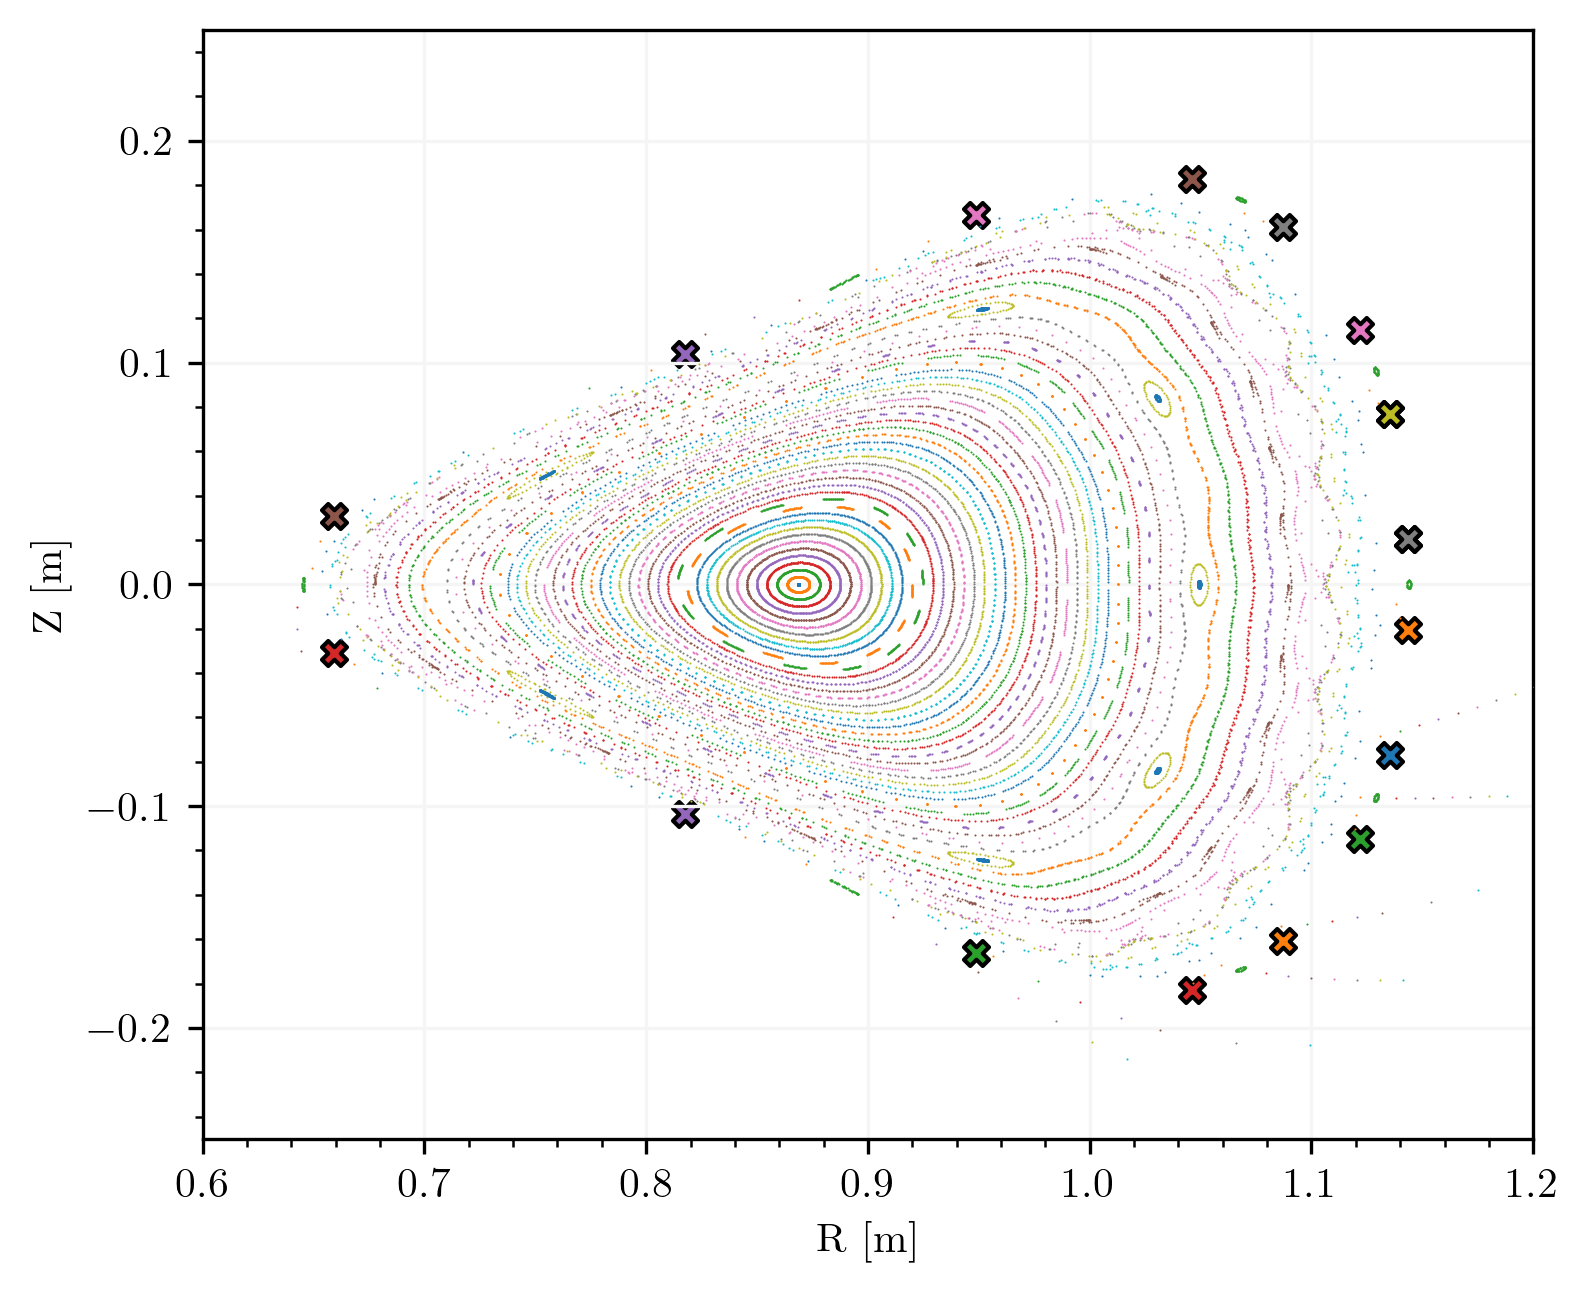
\includegraphics[width=0.7\textwidth]{images/quasrs/fixedpoint_0229079_1.png}
    \caption{Poincaré section at $\phi=0$ of the QUASR configuration 0229079. The X/O fixed points of the island chain $n/m = 6/16$ are drawn as $X$ and $O$ marker.}
    \label{fig:0229079-p}
\end{figure}

\begin{figure}[H]
    \centering
    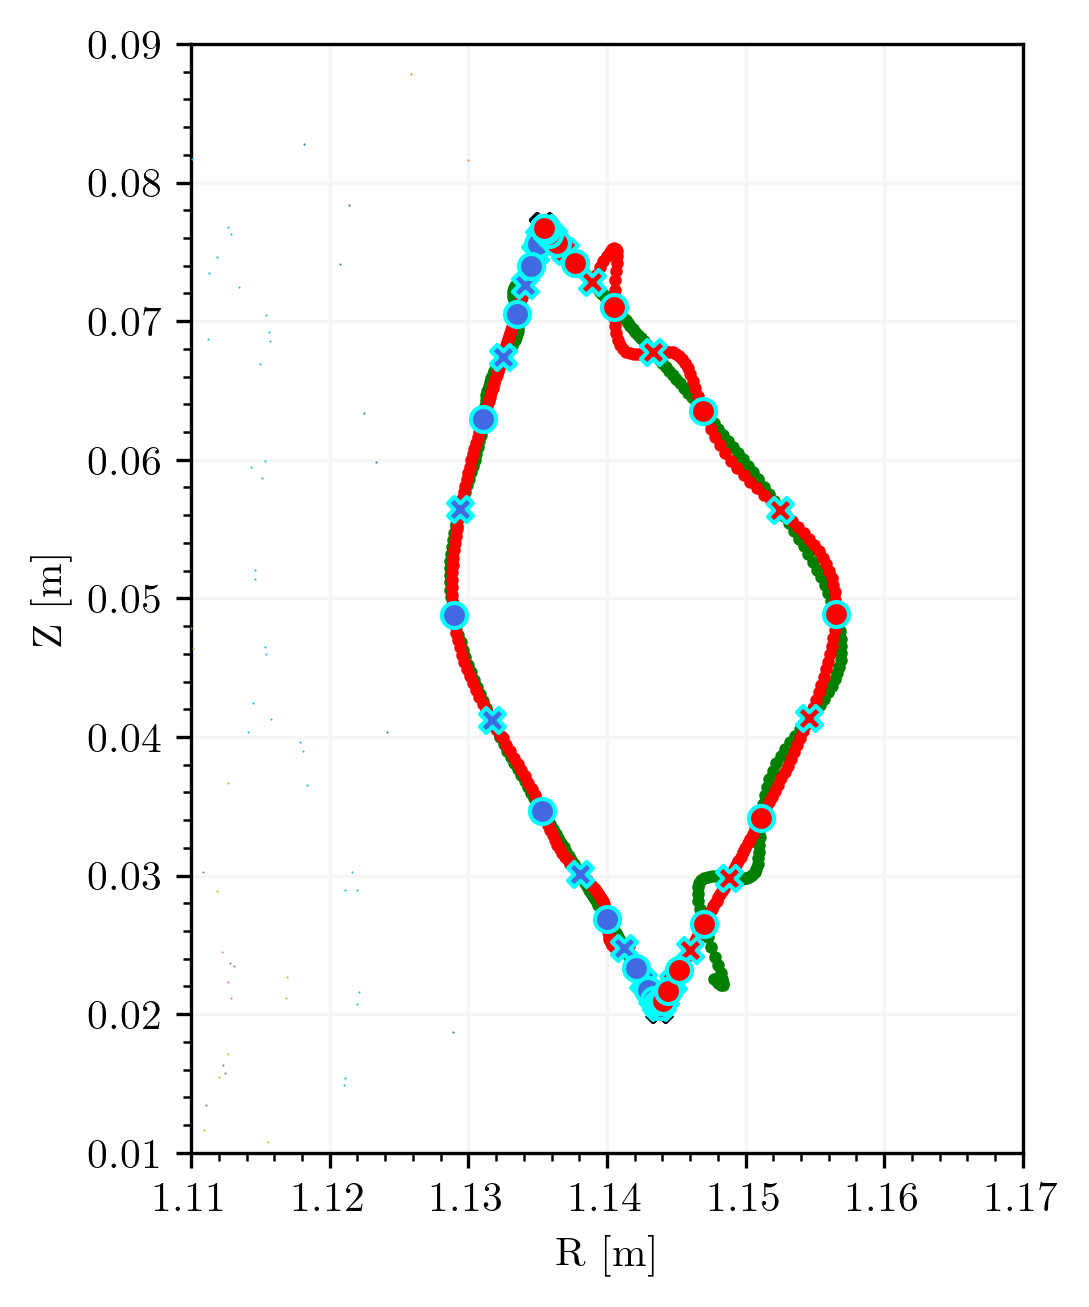
\includegraphics[width=0.5\textwidth]{images/quasrs/clinic_outer_0229079.png}
    \caption{Inner and outer tangle and heteroclinic points for an island crossing of the $n/m  = 6/16$ chain. There are two heteroclinic orbits for which the crossings are indicated by two different markers. The inner homoclinics are coloured blue, the outer ones red.}
    \label{fig:0229079-turn}
\end{figure}

\subsection{Chaotic edge}\label{sec:quars-0928241}

The configuration \href{https://quasr.flatironinstitute.org/model/0928241}{\textcolor{blue}{0928241}} is a three field period quasi-axisymmetric stellarator. It has two coils per field period and the current through them are equal. \figref{fig:coils-0928241} shows their geometry and we see that they are long and wiggly. The rotational transform profile \figref{fig:iota-0928241} goes up from the axis to the edge at first and then goes back down again. The mean value for $\iotaslash$ is 0.5.

\begin{figure}[H]
    \centering
    \begin{subfigure}[t]{0.47\textwidth}
        \centering
        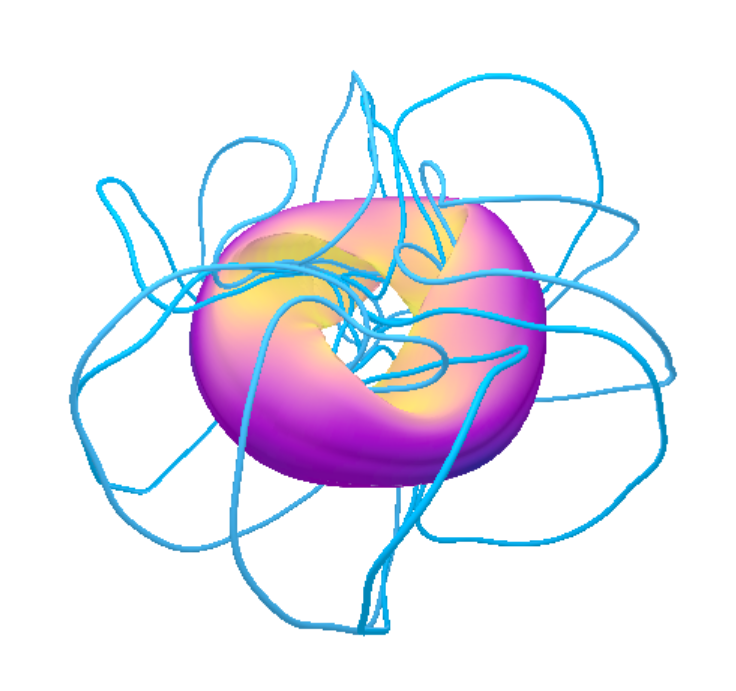
\includegraphics[width=\textwidth]{images/quasrs/config-0928241.png}
        \caption{}
        \label{fig:coils-0928241}
    \end{subfigure}
    \hfill
    \begin{subfigure}[t]{0.52\textwidth}
        \centering
        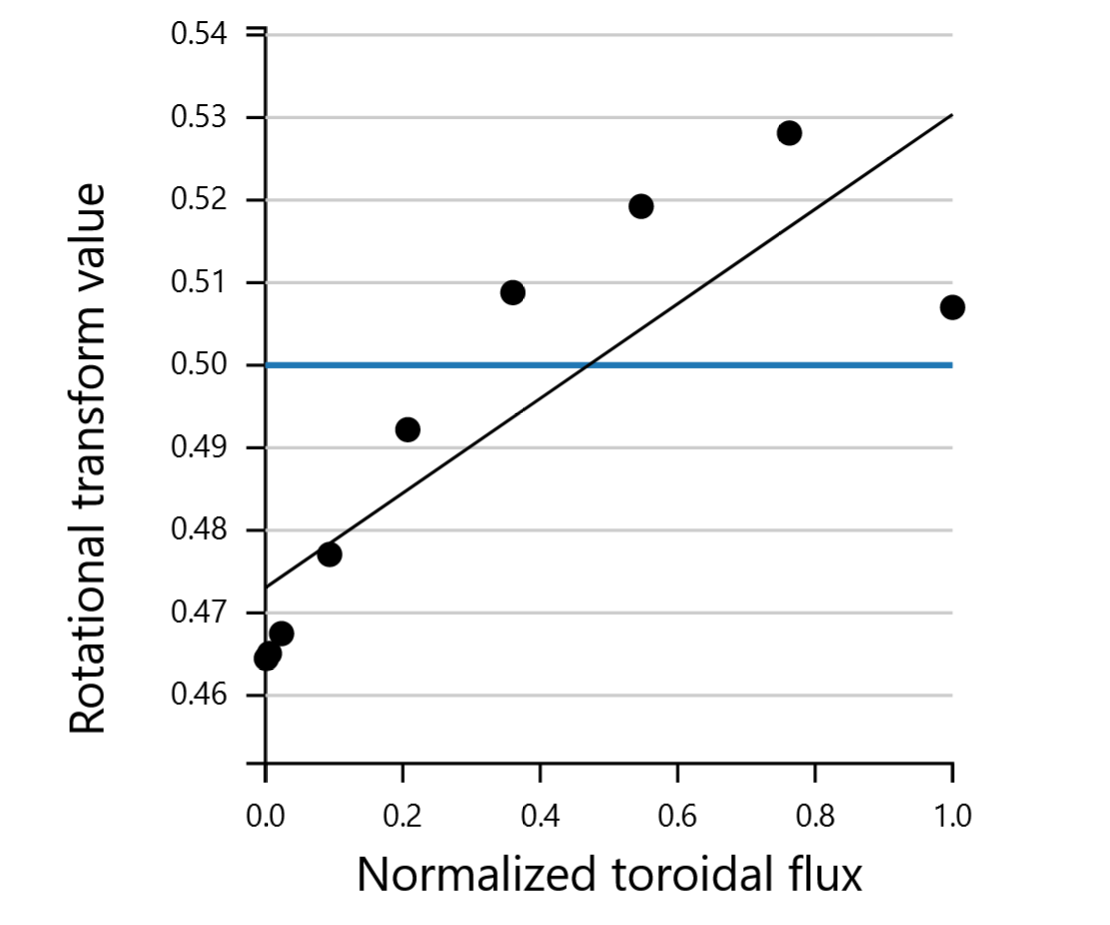
\includegraphics[width=0.8\textwidth]{images/quasrs/iota-0928241.png}
        \caption{}
        \label{fig:iota-0928241}
    \end{subfigure}
    \caption{QUASR configuration 0928241. (a) Coil structure and an external magnetic surface, the same colours indicate the same value of current flowing into the coils. (b) Rotational transform against the normalised toroidal flux and its mean value as a horizontal line.}
    \label{fig:config-0928241}
\end{figure}

\begin{figure}[H]
    \centering
    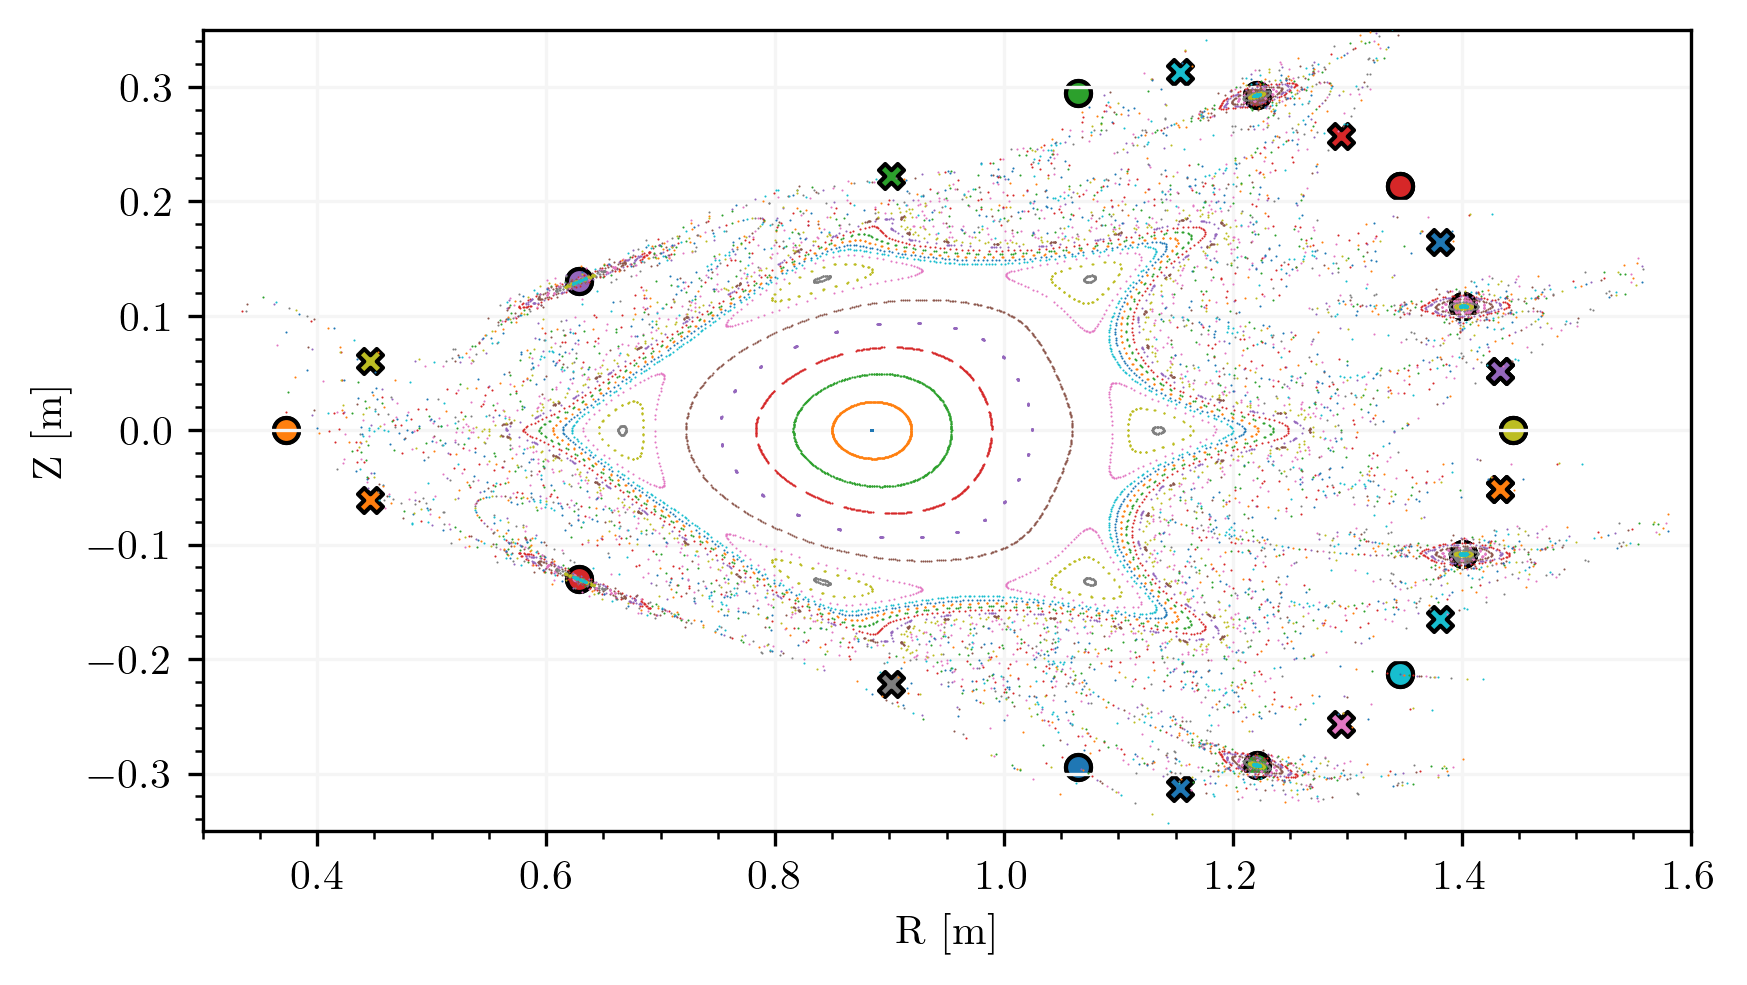
\includegraphics{images/quasrs/fixedpoint_ox_0928241.png}
    \caption{Poincaré section at $\phi=0$ of the QUASR configuration 0928241. The X/O fixed points of the island chain $n/m = 6/12$ are drawn as $X$ and $O$ marker.}
    \label{fig:p-0928241}
\end{figure}


\begin{figure}[H]
    \centering
    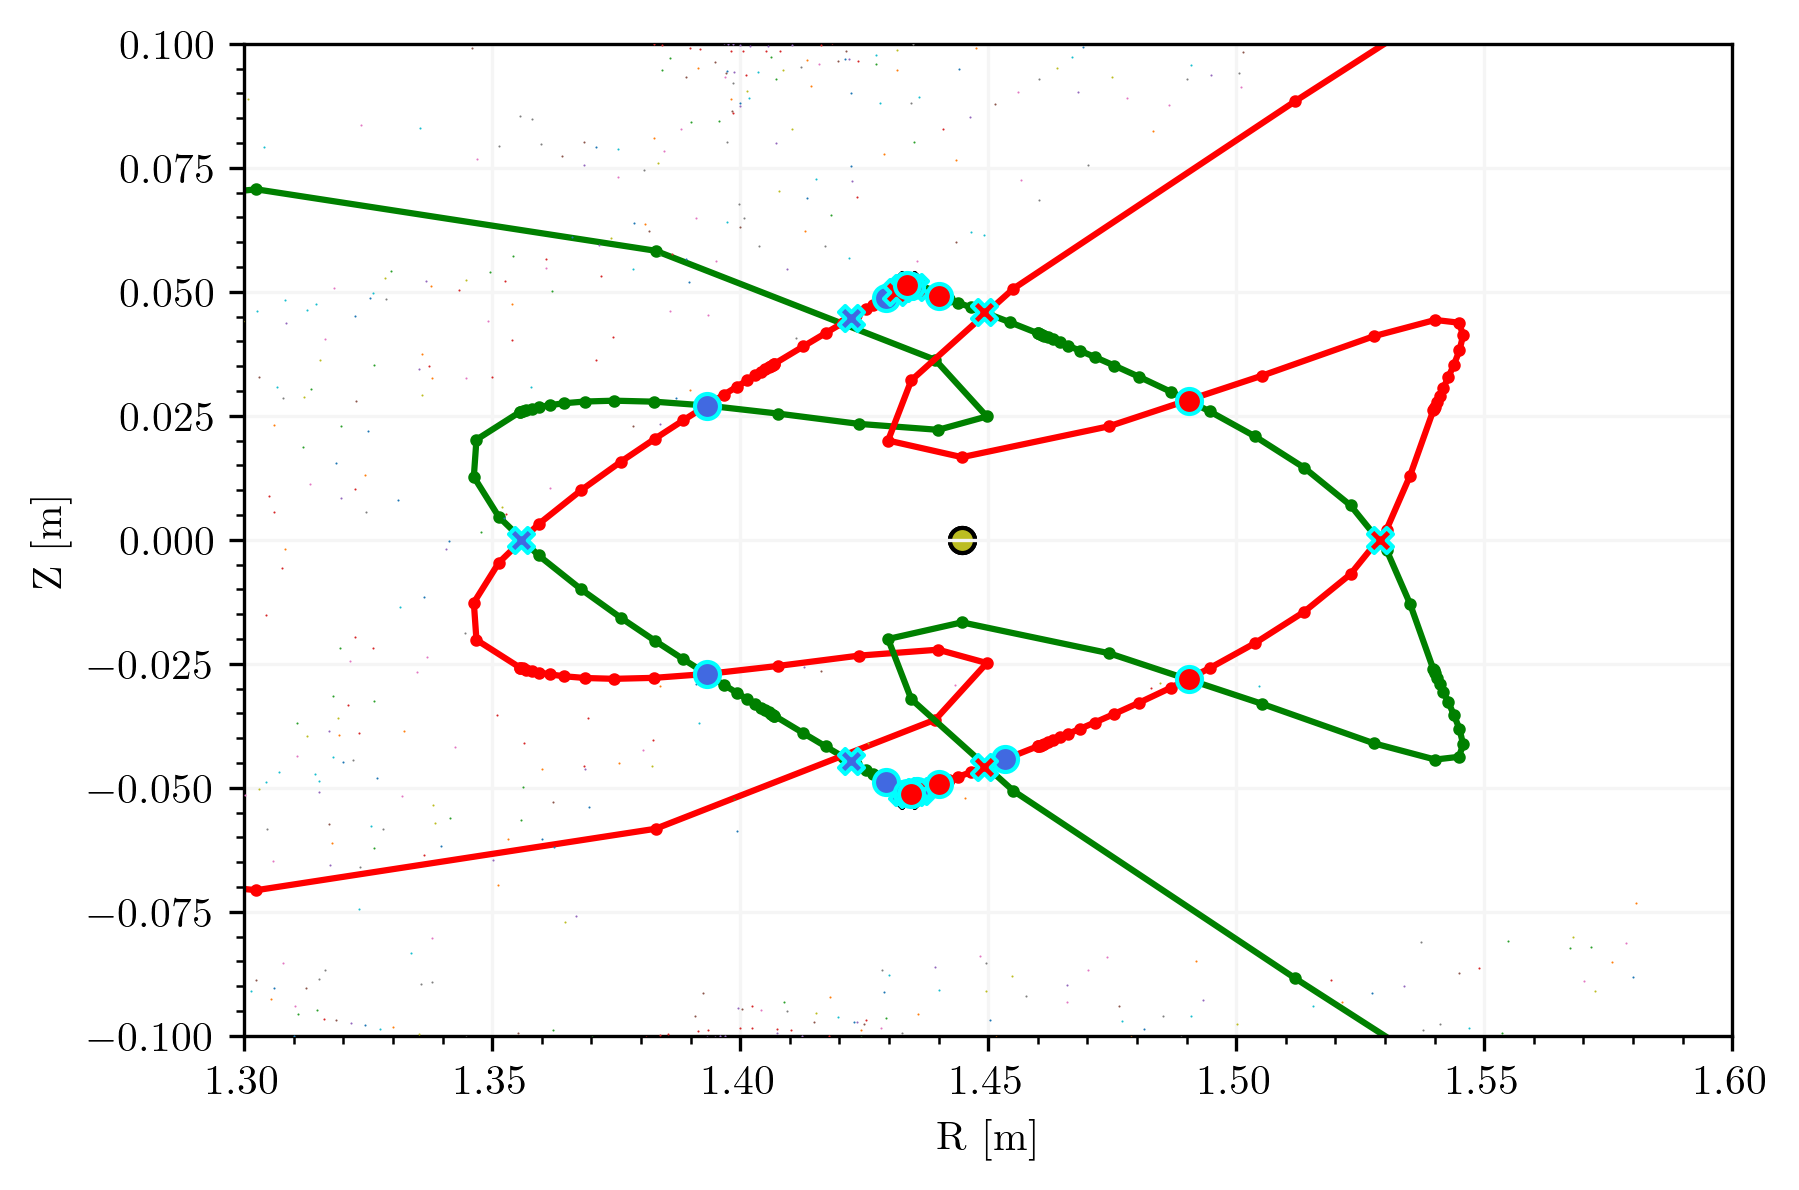
\includegraphics[width=0.8\textwidth]{images/quasrs/outer_0928241.png}
    \caption{Inner and outer tangle and heteroclinic points for an island crossing of the $n/m  = 6/12$ chain. There are two heteroclinic orbits for which the crossings are indicated by two different markers. The inner homoclinics are coloured blue, the outer ones red.}
    \label{fig:turn-0928241}
\end{figure}

The starting point for the FLT where set such that the two islands par of the island chain in the edge could be seen. However, and disturbingly at first, only one of the two has closed surfaces. It could be that the island is super tiny, can it disapear ? 

The fact that O-point are elliptic point is not the best definition. Indeed there is a more topological definition of the difference between O/X-point relying on their topological index. 

By noting this, the case $\lambda_s, \lambda_u < 0$ and $\lambda_s, \lambda_u > 0$ are two distinct point, the second is the usual X-point saddle but the first one is in fact also a different kind of O-point. The first case was as alternating hyperbolic point in \cite{smiet_bifurcations_2020}. Depending on the value of the trace one can differentiate alternating elliptic O-point from elliptic O-point from hyperbolic X-points. The Greene's Residues 

\begin{figure}[H]
    \centering
    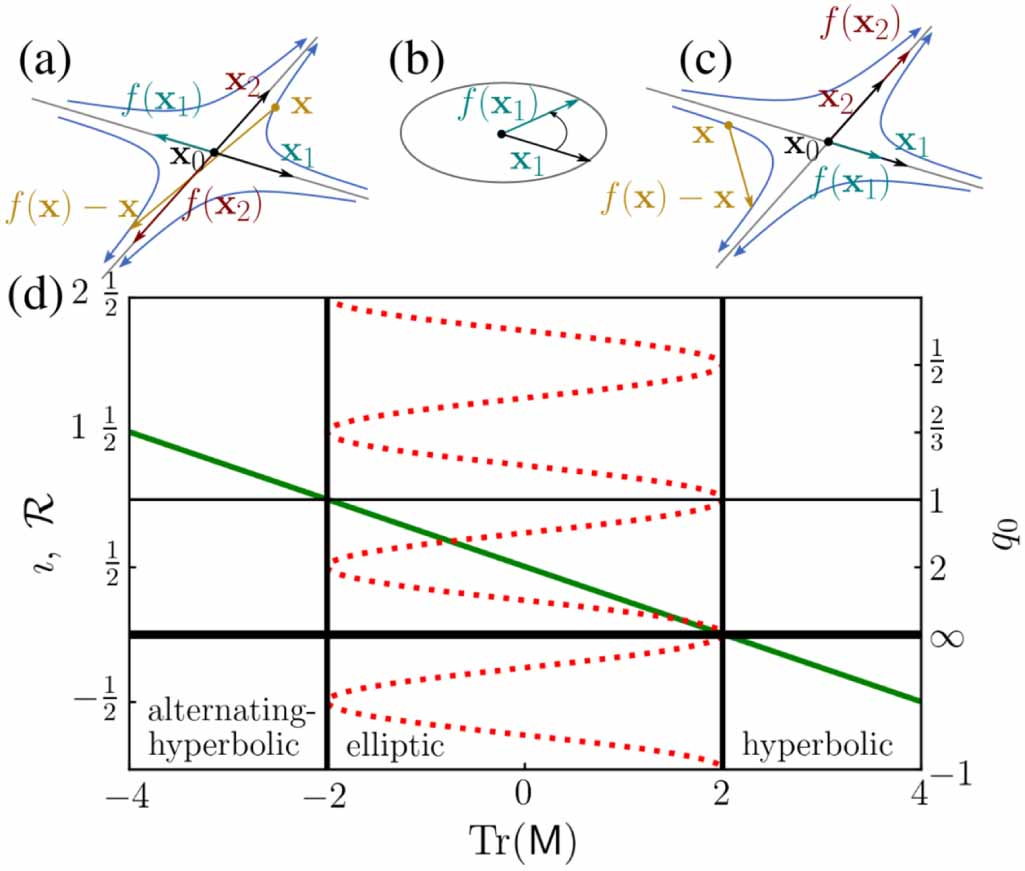
\includegraphics[width=0.6\textwidth]{images/theory/smeit_sawtooth.jpg}
    \caption{Characterization of the fixed point by the value of the trace of the jacobian matrix $\dpmap$ of the field line map (written M here) taken from \cite{smiet_bifurcations_2020}.}
    \label{fig:smeit-bifurcations}
\end{figure}

For the four fixed point found in the $\iotaslash = 6/12$ island chain are regrouped in \tabref{tab:greenes}. Point 1 and 2 correspond have 
\tabref{tab:greenes} gives the Greene's Residue $\mathcal{R} = \frac{1}{2} - \frac{1}{4}\text{Tr}(\dpmap^k\vert_{\z^\star})$, for the 4 fixed points orbits of the $6/12$ island chain and with the def of sec we see that while the point 1 and 2 are indeed hyperbolic fixed point X-point with the same value of the residue $\mathcal{R} < 0$. But the point 3 and 4 are O-point but actually point 3 is indeed an elliptic O-point but the 4 point has residue $0 < \mathcal{R}(3) < 1$ which means that it is an altearnating fixed point ! Here there is in fact a tangle structure around another tangle structure which would be a mobius strip ! The chaos is much more present in the inside of this region for the alternating hyperbolic due to the presence of an third tangle structure on the inside of the resonance zone itself !

\begin{table}[H]
    \centering
    \begin{tabular}{c|c|c|c|c}
         & 1 & 2 & 3 & 4 \\
         \hline Residue $\mathcal{R}$ & -2.16 & -2.16 & 1.10 & 0.55
    \end{tabular}
    \caption{Greene's residue calculated for each of the four fixed point orbits in the 6/12 island chain. The two X-points have the same value for $\mathcal{R} = \mathcal{R}_1 = \mathcal{R}_2$. The two O-points, however, have different values for their residue.}
    \label{tab:greenes}
\end{table}

\subsection{Large island}\label{sec:quars-1329594}

The last QUASR configuration which will be looked at is the configuration \href{https://quasr.flatironinstitute.org/model/1329594}{\textcolor{blue}{1329594}}

In \figref{fig:config-1329594}, the coil configuration is shown. The coil structure is really intricated. It seems like the field periodicity is equal to six but in fact it is equal to 3. the number of coil per field period is two and the . it is a quasi-helically symmetric stellarator. Its aspect ratio is of 9.97. 

It was looked for high mean $\iotaslash$ which is the case here at a value of 1.8 and in fact it is surely why this almost looks like a $\nfp = 6$ device. indeed a high iota value mean more twisting, therefore doing the turn taking a nfp = 3 and doubling it is kind of what happens. The iota profile calculation has only four points which is not much and only one in the edge. it goes from about 1.84 to 1.76 at the edge.

\begin{figure}[H]
    \centering
    \begin{subfigure}[t]{0.49\textwidth}
        \centering
        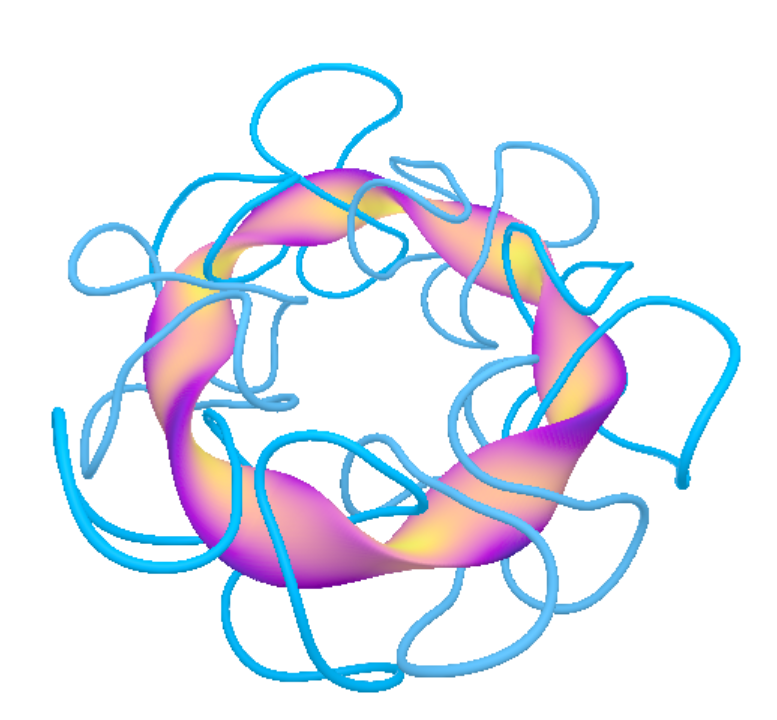
\includegraphics[width=\textwidth]{images/quasrs/config-1329594.png}
        \caption{}
        \label{fig:coils-1329594}
    \end{subfigure}
    \hfill
    \begin{subfigure}[t]{0.49\textwidth}
        \centering
        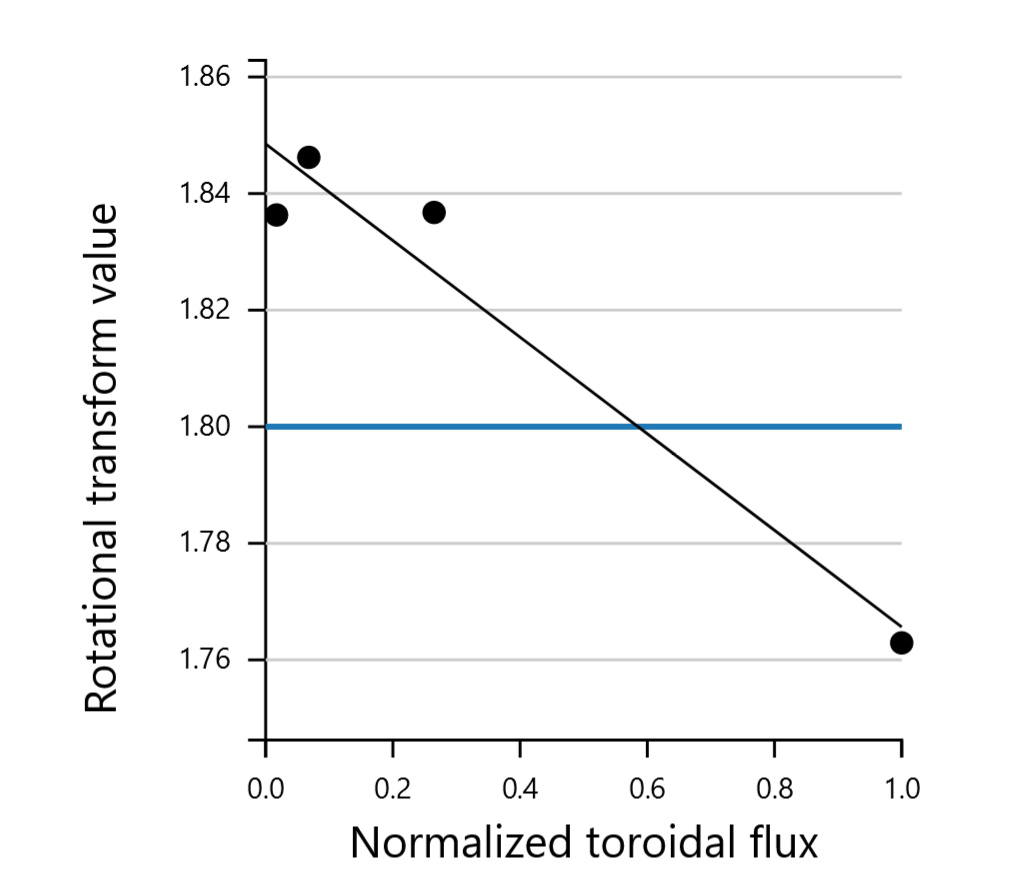
\includegraphics[width=0.8\textwidth]{images/quasrs/iota-1329594.png}
        \caption{}
        \label{fig:iota-1329594}
    \end{subfigure}
    \caption{QUASR configuration 1329594. (a) Coil structure and an external magnetic surface, the same colours indicate the same value of current flowing into the coils. (b) Rotational transform against the normalised toroidal flux and its mean value as a horizontal line.}
    \label{fig:config-1329594}
\end{figure}

\figref{fig:p-1329594} shows the Poincaré section. The island is of the order of a third of the main region and the profile is really elongated. Only one orbit does all the crossings and the island is a $n/m = 3/5$. It is not a clear relation with the iota profile, it may also be that this device in reality a $\nfp = 6$ device for which the optimization was set for a nfp = 3 and which gave back this. This would mean that the $\iotaslash = 6/5 = 1.2$ which may be more realistic.

Nevertheless the the turnstiles are small compared to the size of the island and the configuration has very little chaos. An optimization could still try to reduce the chaos further by shaping the coils or adjusting the current just a little bit to make this turnstiles, and in particular the outer one smaller. Or to maybe to combine a somewhat big island with a bigger turnstile to. The question is do we want or not chaos here for instance but we are now able to make it more or less chaotic.

\begin{figure}[H]
    \centering
    \begin{subfigure}[t]{\textwidth}
        \centering
        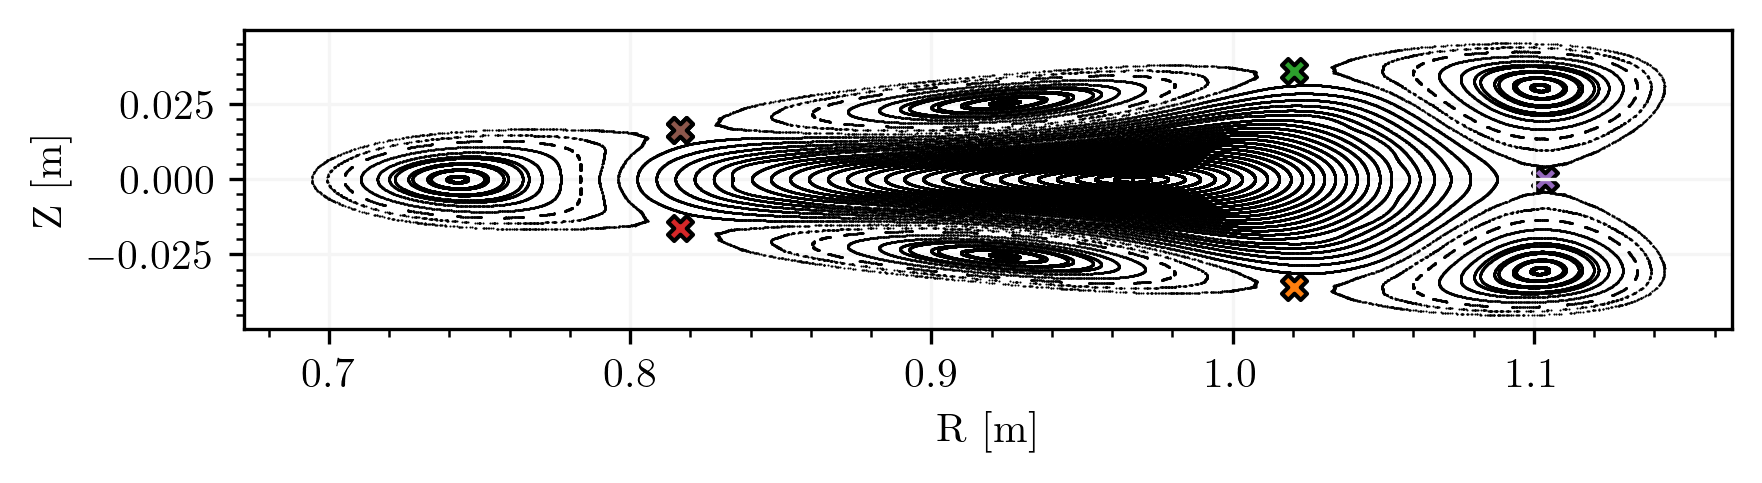
\includegraphics[width=\textwidth]{images/quasrs/poincare_1329594.png}
        \caption{}
        \label{fig:p-1329594}
    \end{subfigure}
    \begin{subfigure}[c]{0.54\textwidth}
        \centering
        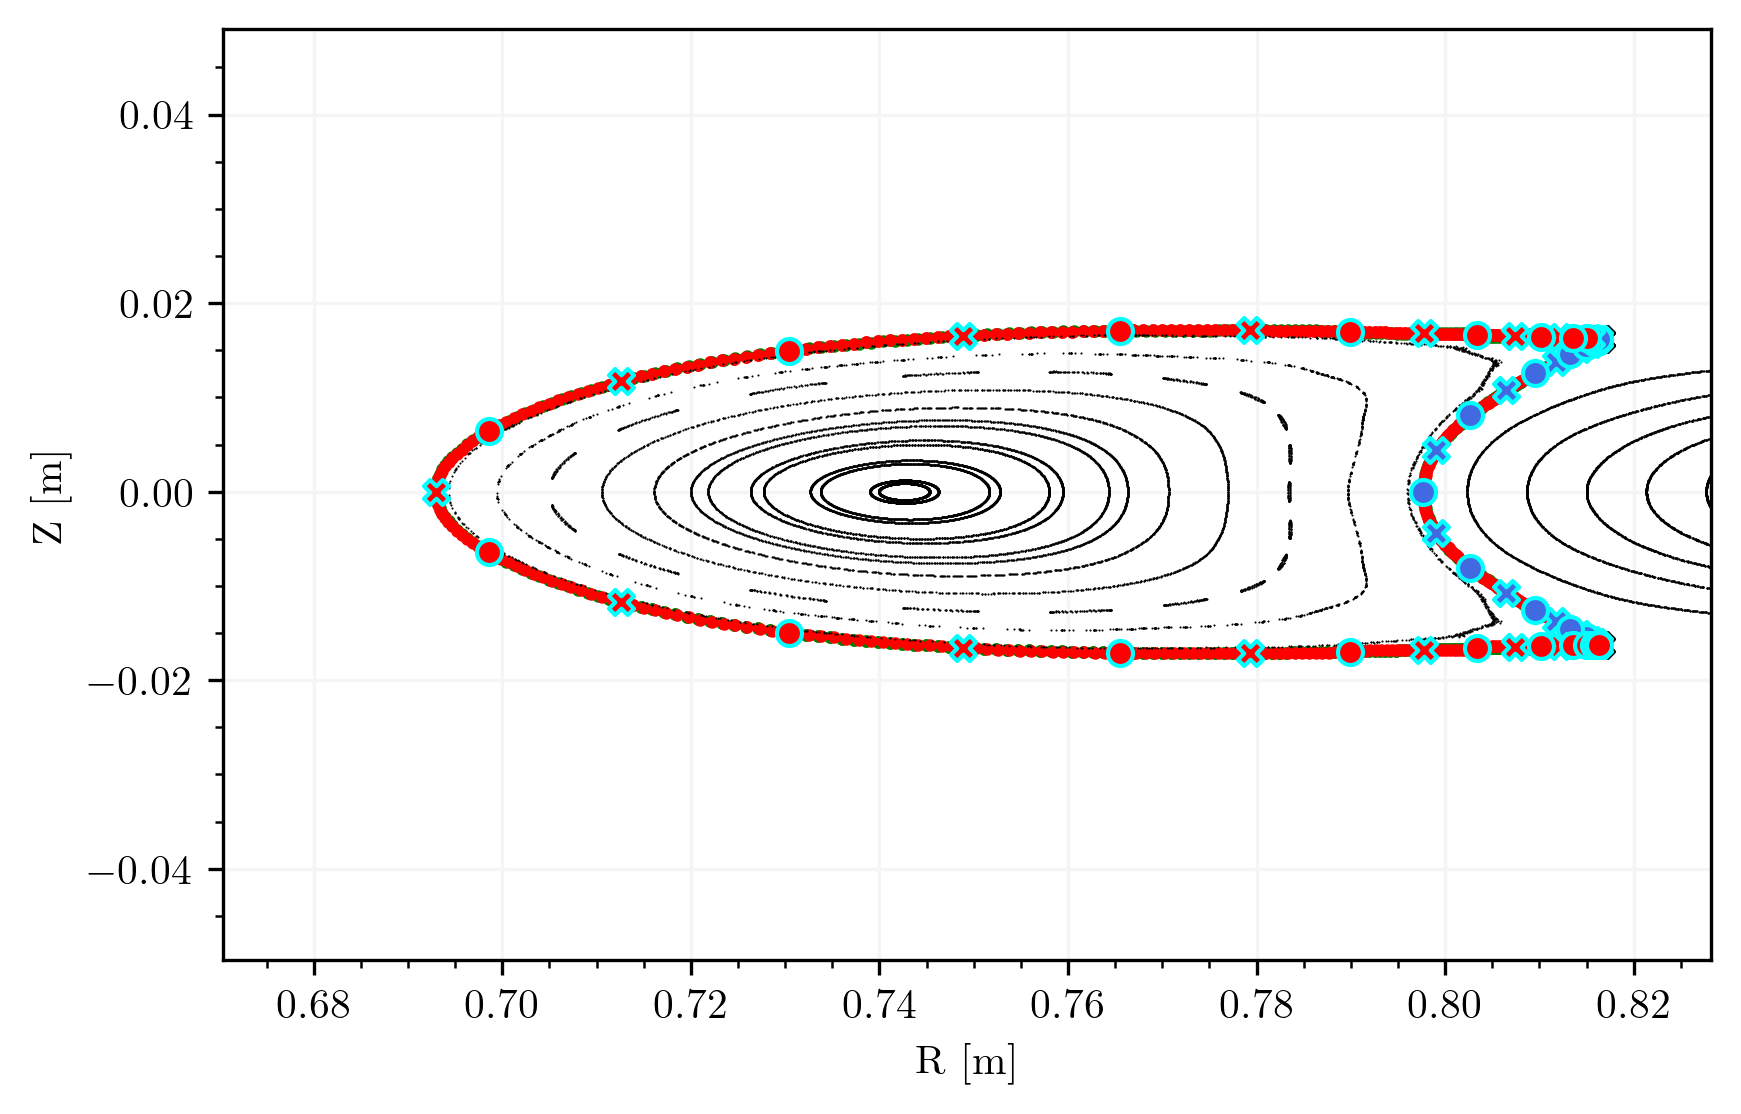
\includegraphics[width=\textwidth]{images/quasrs/homoclinics_1329594.png}
        \caption{}
        \label{fig:manifold-1329594}
    \end{subfigure}
    \hfill
    \begin{subfigure}[c]{0.44\textwidth}
        \centering
        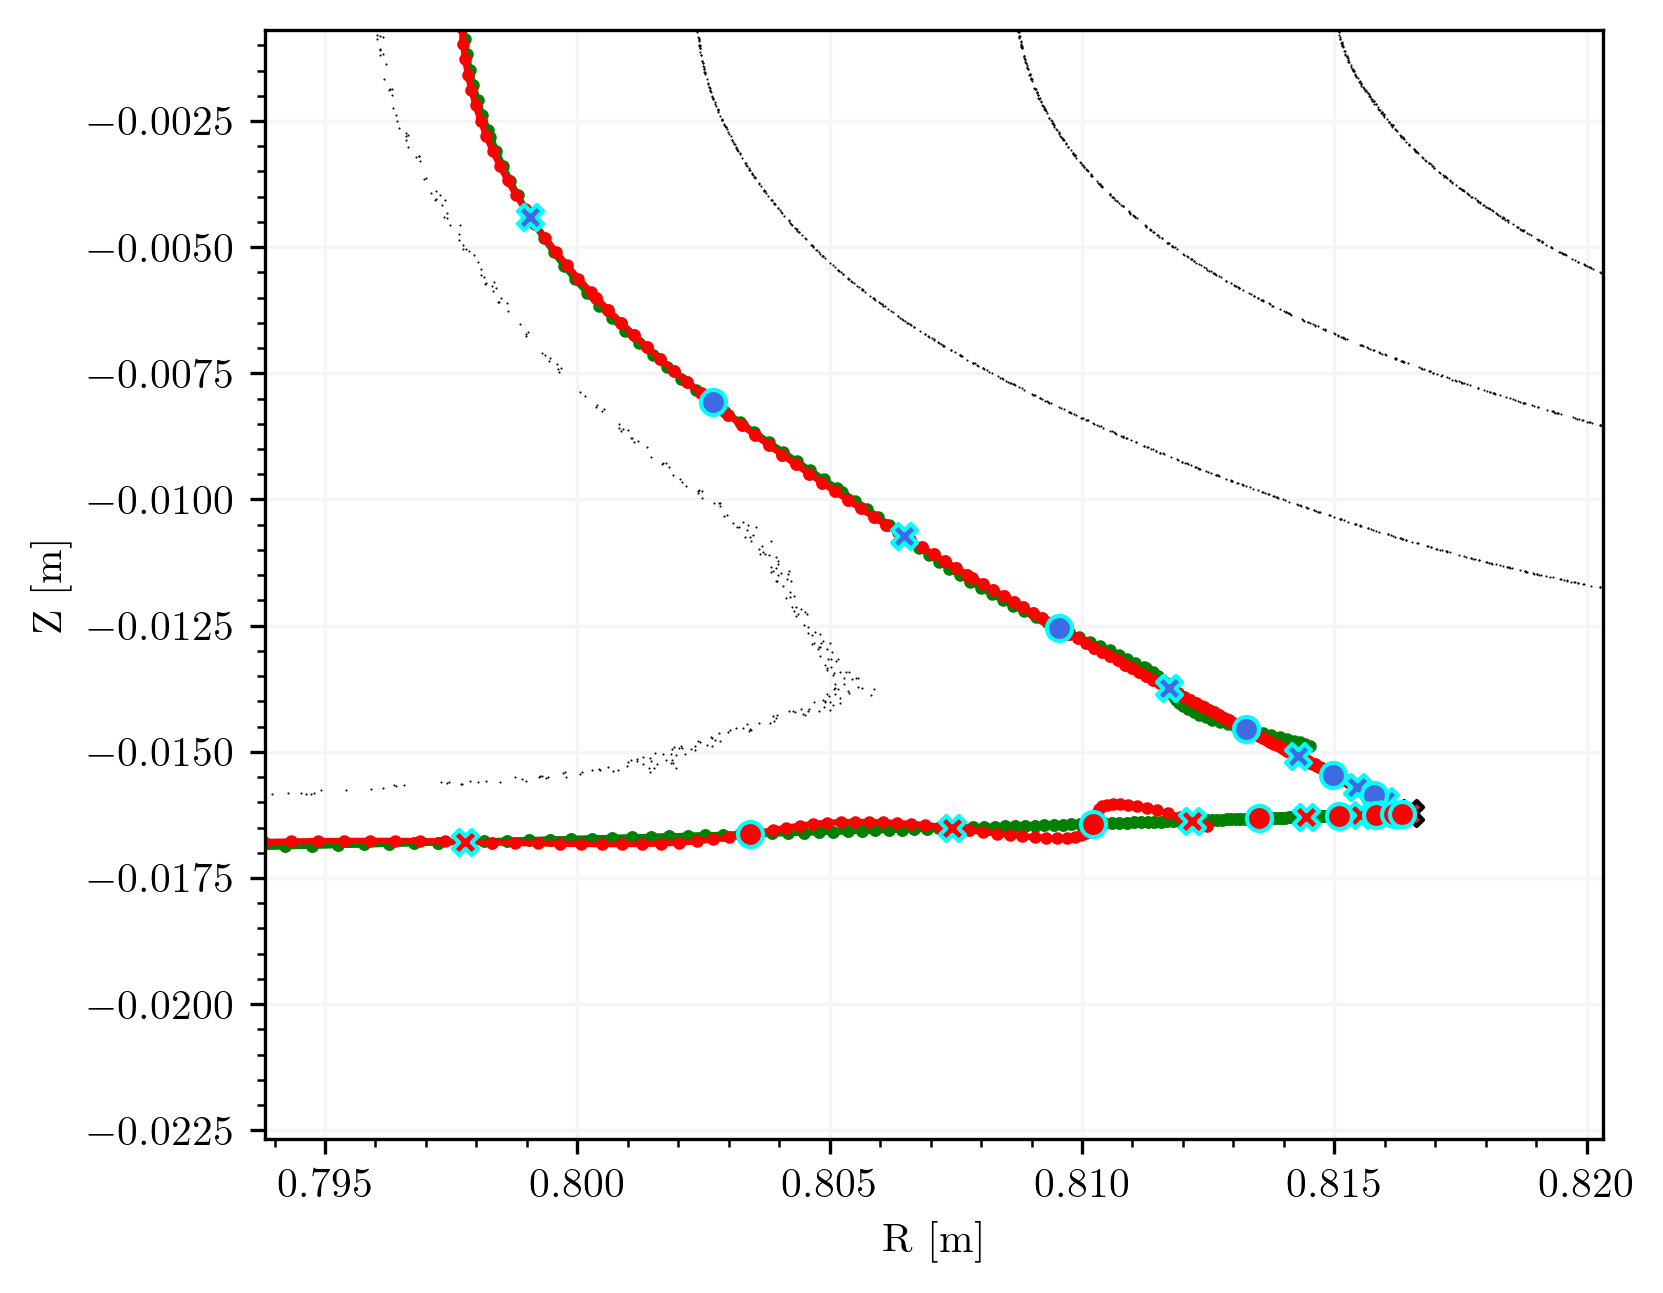
\includegraphics[width=\textwidth]{images/quasrs/homoclinics_1329594_cu.png}
        \caption{}
        \label{fig:turn-1329594}
    \end{subfigure}
    \caption{Poincaré section at $\phi=0$ of the QUASR configuration 1329594 in (a) with the X-points of the of island $n/m = 3/5$ drawn as $X$ marker. In (b) : look at the manifold structure around the left island crossing. In (c) : closer around the lower X-point of the island. The two heteroclinic orbits are indicated by distinct markers : circles and crosses. The inner ones are coloured in blue, the outer ones in red.}
    \label{fig:pmt-1329594}
\end{figure}

\section{Wendelstein 7-X}\label{sec:w7x}

Wendelstein 7-X is a 5 field period device with a total of 50 modular coils located in Greifswald, Germany. Per field period, in addition to the 10 modular coils that generate the standard W7X field, 4 planar coils can be used to further vary the magnetic field. In this existing stellarator experiment, the shape of the coils is difficult, if not impossible, to alter. The current, on the other hand, can be easily adjusted to vary the magnetic topology.

The standard configuration, shown in \figref{fig:w7x-default}, is obtained by running a current of 1.62 MA in the modular coils and none in the planar coils. This configuration of W7X was designed to be non-chaotic and exploits the 5/5 island chain in the edge as an island divertor concept. However, other more chaotic configurations can be explored. By reducing the currents in the modular coils to 1.1095 MA and those in the planar coils are set to -0.3661 MA creates the GYM00-1750 obtained by Robert Davies. Its Poincar\'e section \figref{fig:gym00-poincare} displays a smaller $n/m = 5/4$ island and a chaotic edge region.

\begin{figure}[H]
    \centering
    \begin{subfigure}[c]{0.51\textwidth}
        \centering
        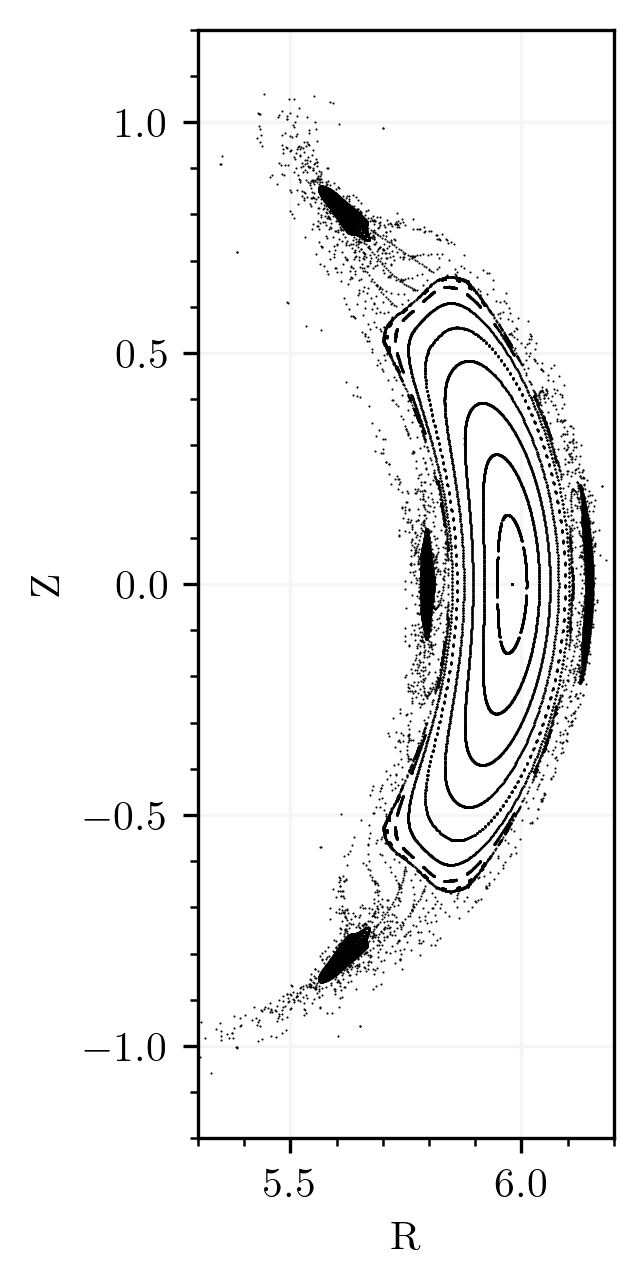
\includegraphics[width=0.8\textwidth]{images/w7x-gym00-1750/gym00_1750.png}
        \caption{}
        \label{fig:gym00-poincare}
    \end{subfigure}
    \hfill
    \begin{subfigure}[c]{0.47\textwidth}
        \centering
        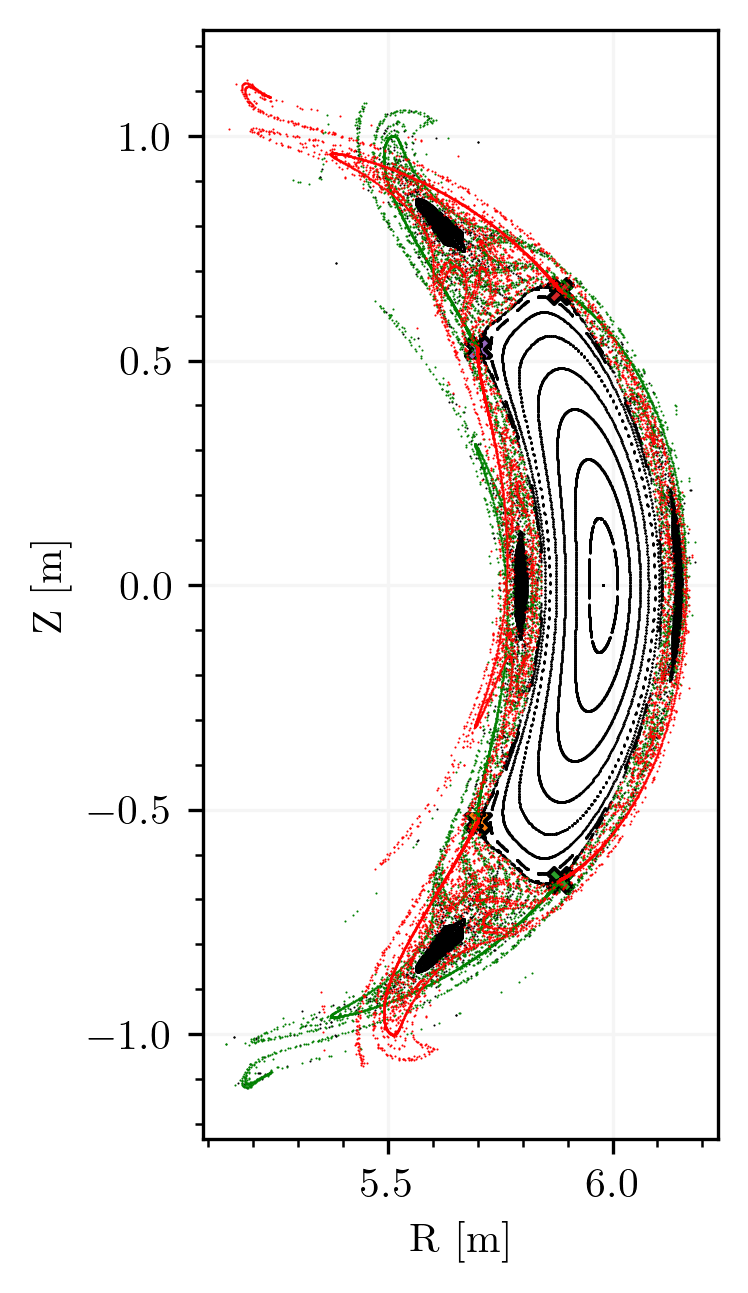
\includegraphics[width=\textwidth]{images/w7x-gym00-1750/gym99_1750_fixedpoints.png}
        \caption{}
        \label{fig:gym00-tangles}
    \end{subfigure}
    \caption{Wendelstein 7-X chaotic GYM00-1750 configuration Poincaré plot (a) and tangle structure with heteroclinics in (b). A $n/m=4/5$ island can be observed and chaos is present in the edge.}
    \label{}
\end{figure}

The tangle structure created by the stable and unstable manifold is shown in \figref{fig:gym00-tangles}. The complex lattice structure intersects many times and the primary heteroclinics are nicely located. In this context, in order to trace $W^s$ and $W^u$ with higher precision, the field is evaluated directly from the Biot-Savart law and the integration is carried out, again using Runge-Kutta Dopri5, with a relative tolerance of 1e-14. However, after a small time evolution, the initial segment still becomes a fuzzy layer and not a perfect 2d line. Tuning the integrator to the device or perhaps using a different integration scheme may help reduce the fuzziness and make the tangles clearer. Although not to be trusted blindly, the Runge-Kutta algorithm is very robust for many ODE systems and is relied upon here.

A field line starting inside the magnetic island will always remain within a confined region of the Poincaré section. A field line from the chaotic layer, on the other hand, will eventually be ejected very far and end up hitting the plasma-facing components. The connection length $L_C$ plot \ref{fig:cl-a} shows this difference in the behaviour of the field lines. The distance travelled before hitting the PCF, i.e. before hitting the computational boundary surface that terminates the integration, is displayed. Higher values therefore mean a longer confinement time and are indicated by a more yellow colour.

we set only points inside so there is only the exits set from forward and backward which are of "use" !

An interesting structure emerges by looking around the island, the connection length is high in certain local regions and then low in its neighbours. Several layers of connection length intensities can also be distinguished. Putting in relation \ref{fig:gym00-tangles} and \figref{fig:cl-a} gives \figref{fig:cl-b} where it can be observed that the tangle structure is identical, and in fact defines, the different connection length zones. The fact that the stable and unstable manifolds are the boundary of these zones brings us back to thinking about the definition of exit and entry sets. Remember that a point in the exit set will be mapped out of the resonance zone (the island) while a point in the entry set will be mapped in. As both forward and backward integration are included there are in fact two entering and two exiting sets $\pmap(E)$, $\pmap(E)$ for forward and $\pmap(E)$$\pmap(E)$ for backward. but the points are initalized only on the inside.

Exiting the resonance zone takes the field line to a the sea that goes to the edge quickly and resutlts in a small connection length $L_C$. The lobes inside of the resonancne zone are also subdivided by the trellis/tanlge structure of the manifold and take diff amount of mapping you need before actually ending up in the particular exiting-entering set and switching from being in the confined region to being on the outside of the resonance zone and going to the edge.

\begin{figure}[H]
    \centering
    \begin{subfigure}[c]{0.48\textwidth}
        \centering
        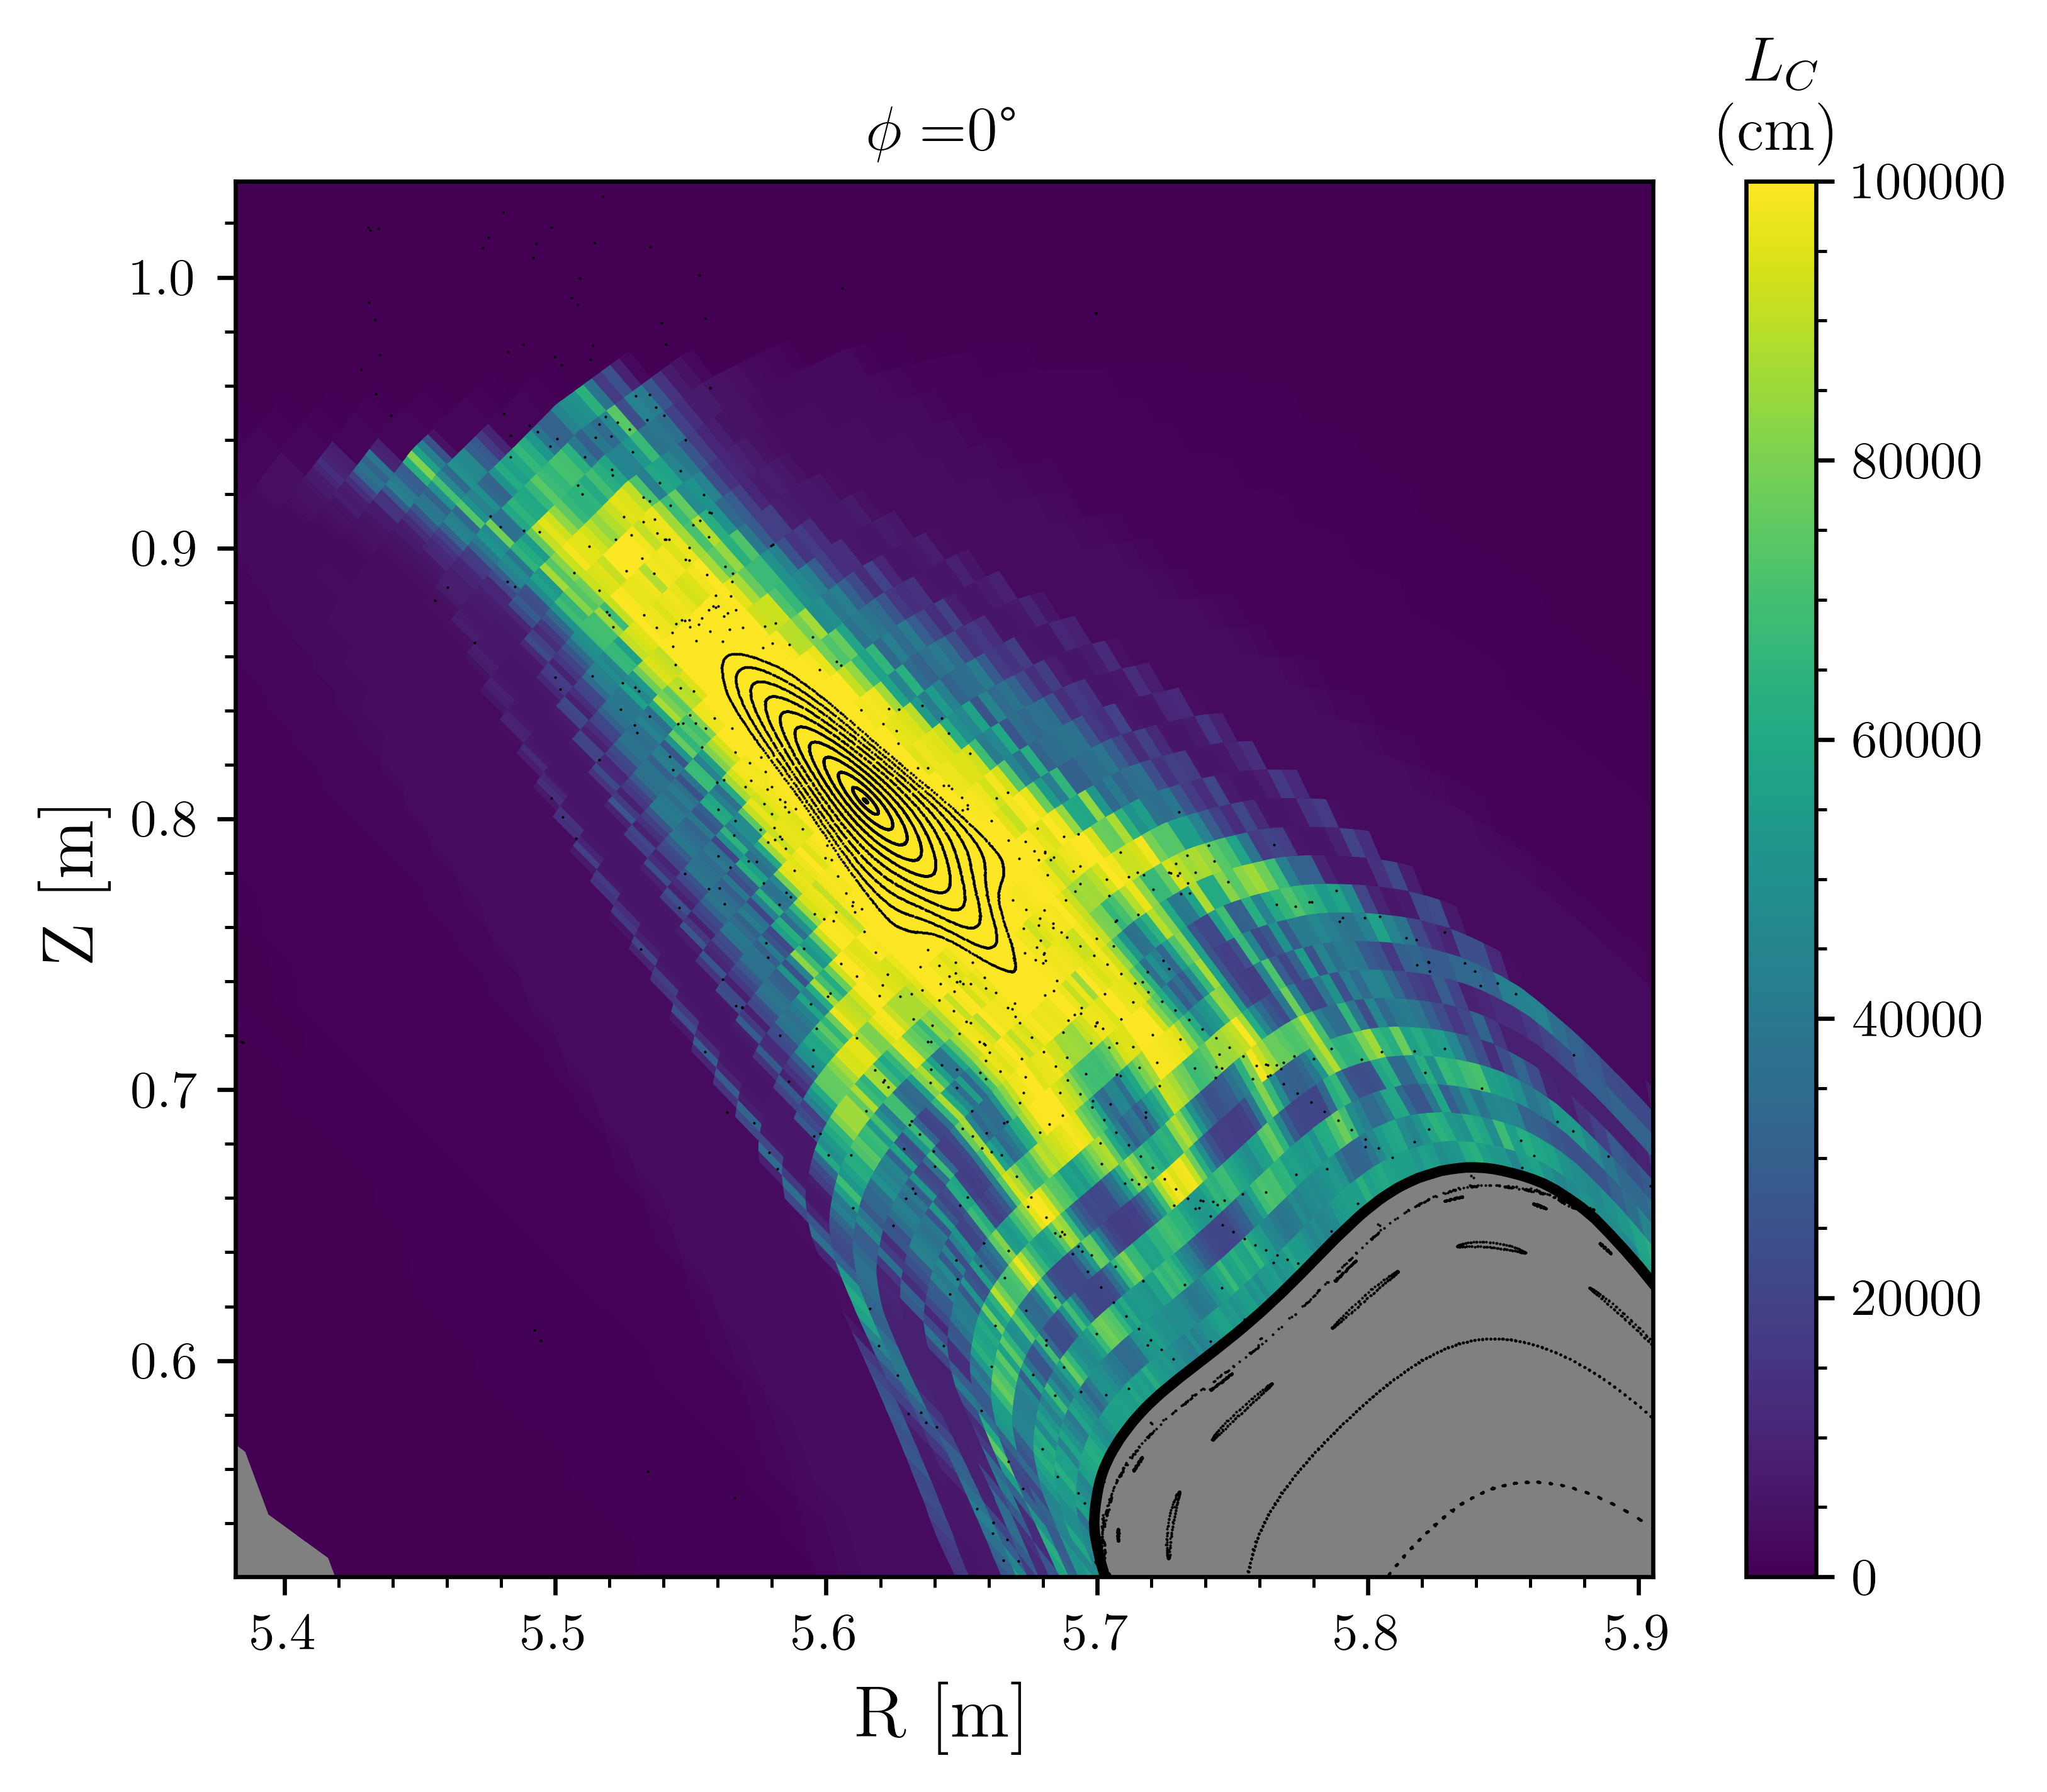
\includegraphics[width=\textwidth]{images/w7x-gym00-1750/gym00_1750_cnpoints.png}
        \caption{}
        \label{fig:cl-a}
    \end{subfigure}
    \begin{subfigure}[c]{0.5\textwidth}
        \centering
        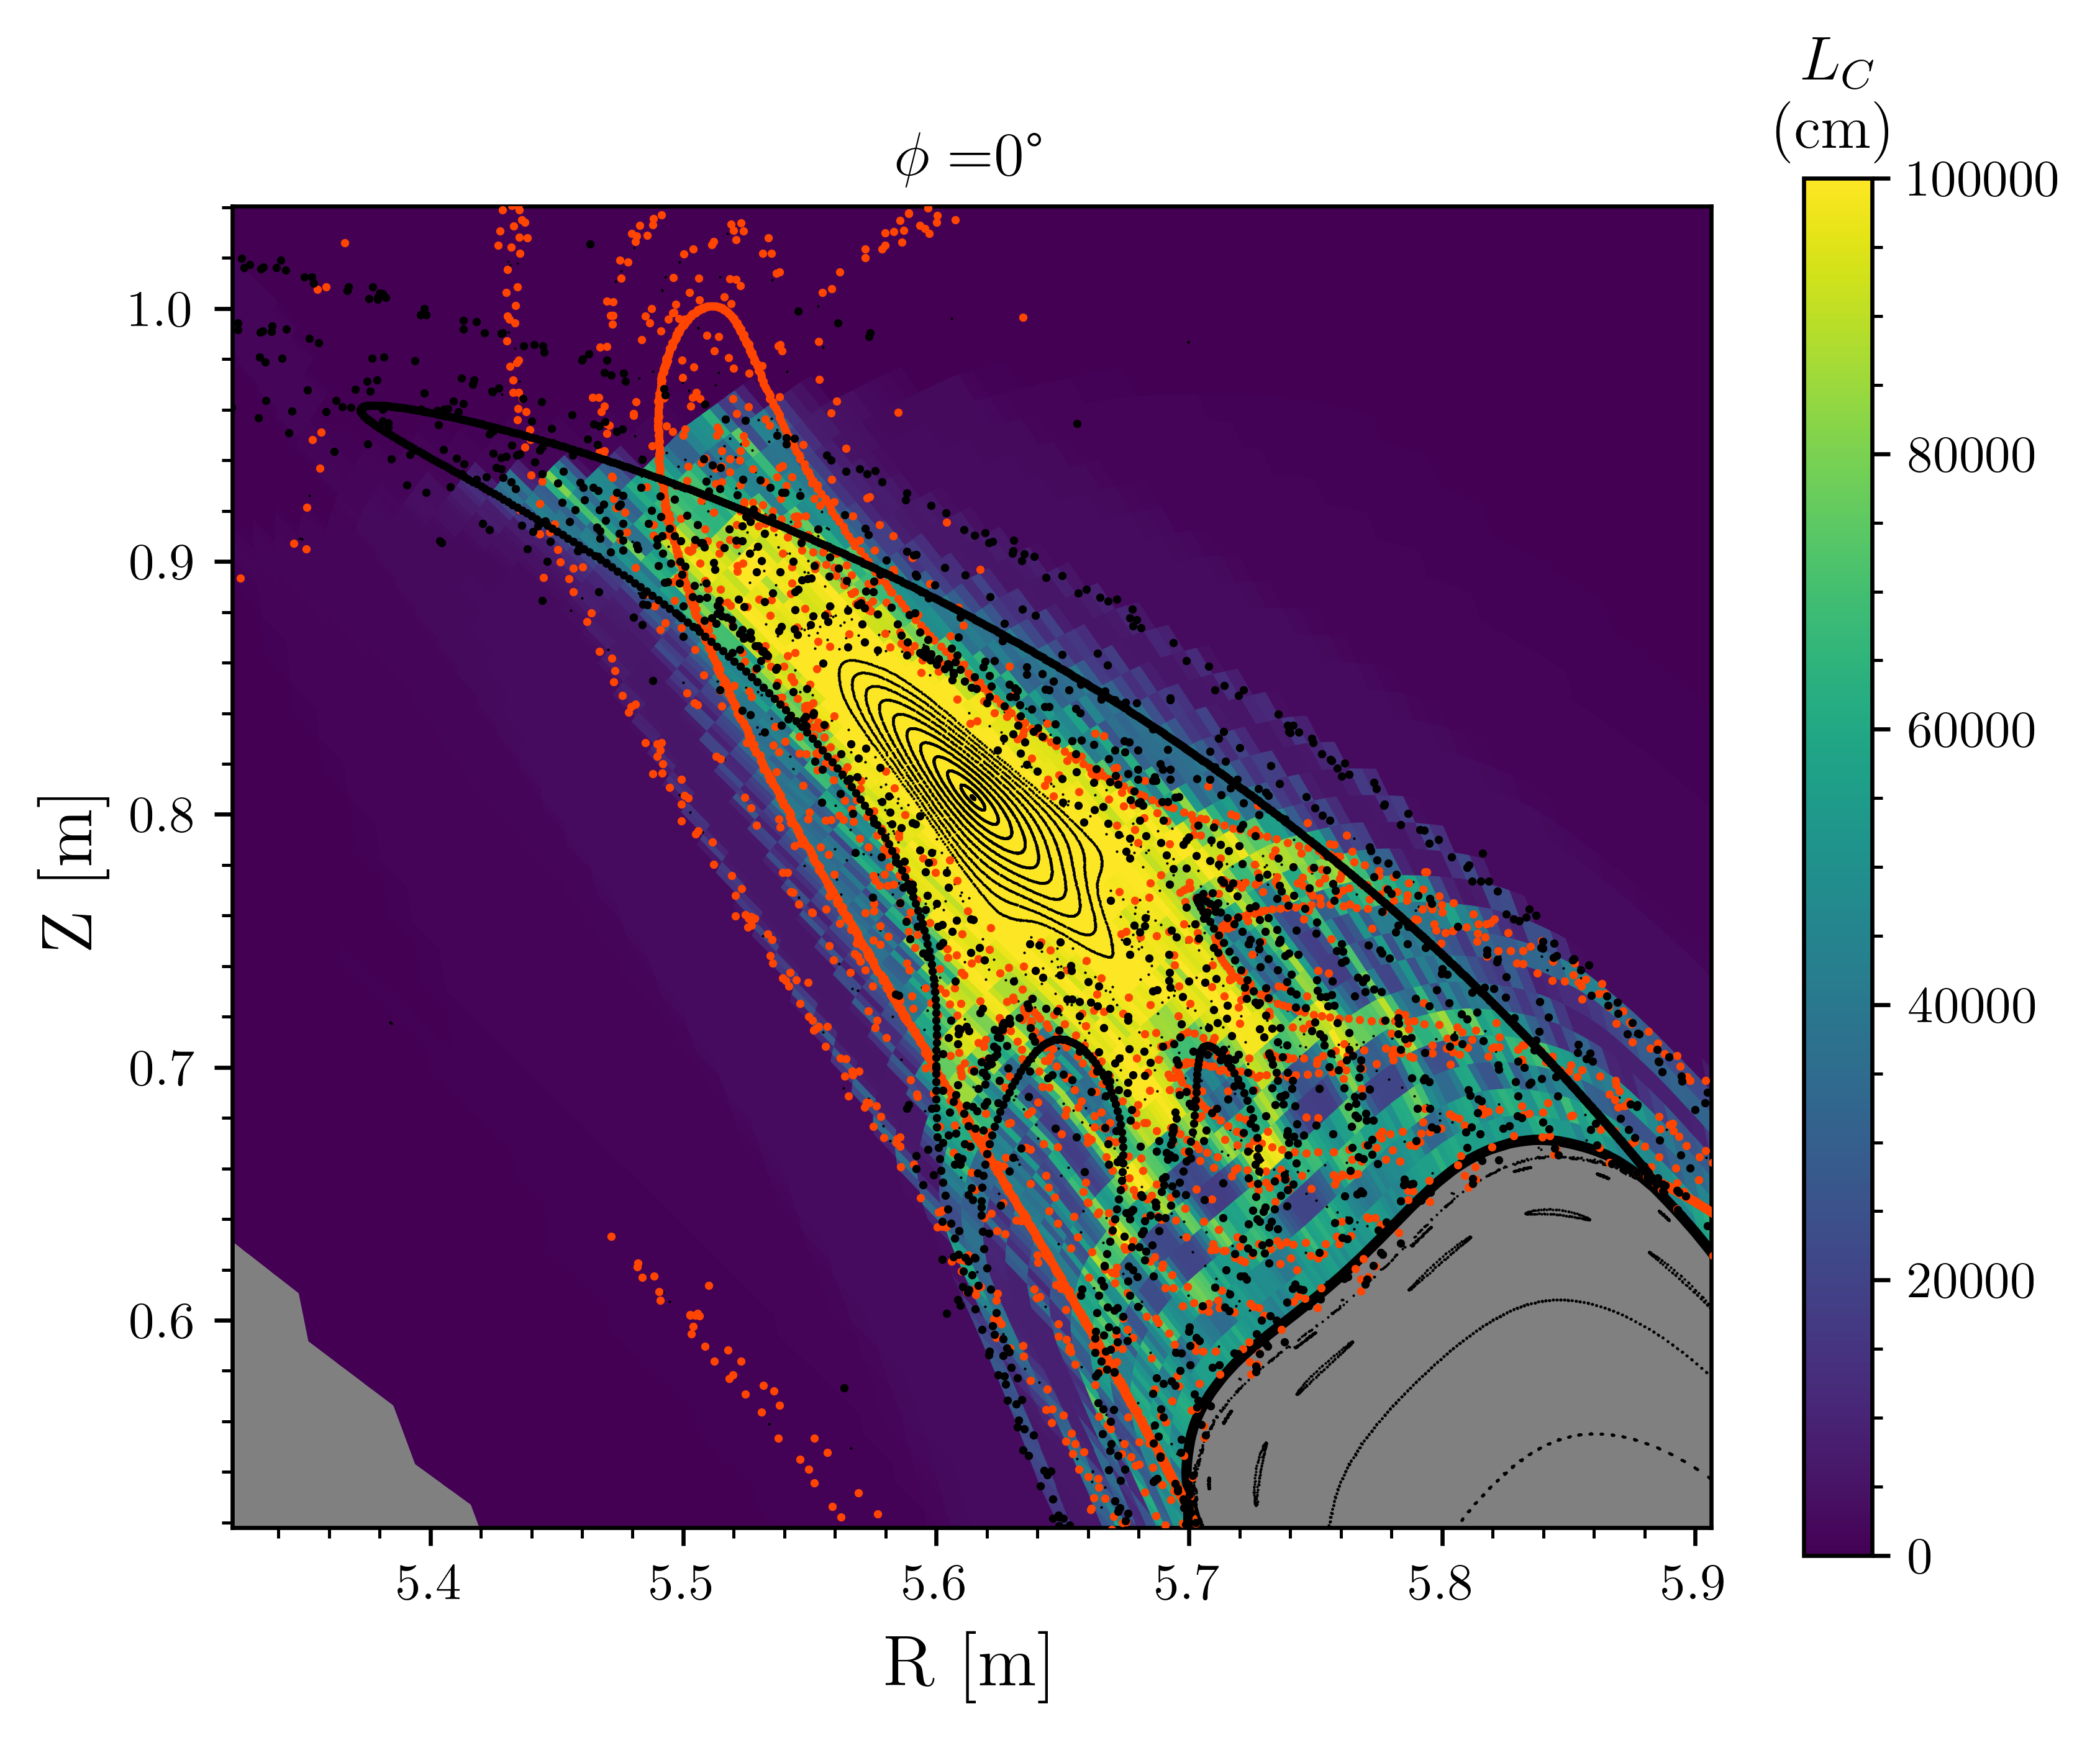
\includegraphics[width=\textwidth]{images/w7x-gym00-1750/gym00_1750_points.png}
        \caption{}
        \label{fig:cl-b}
    \end{subfigure}
    \caption{Minimum connection length between backward and forward tracing for the chaotic W7-X configuration, computed using EMC3-Lite. In (a) around the top island crossing and in (b) superimposing the computation of the manifolds of the saddle.}
    \label{fig:connection-length}
\end{figure}

\section{Inner and outer turnstile fluxes}

The turnstile fluxes have been calculated for the tangles of the specific island considered in each of the configurations presented. In magnetic islands, there is a tangle closest to the magnetic axis, the inner or inner tangle, and a tangle farthest from the axis, the exterior or outer tangle. \tabref{tab:inner-outer-fluxes} gives the flux calculated for the inner and outer turnstiles for each configuration, normalised by the toroidal component of the magnetic field evaluated at the axis $\tilde{B}_0^\phi$. The value of the inner turnstile fluxes are, for all the magnetic fields analysed here, lower than for the outer turnstiles. In the case of the chaotic W7X configuration it is even of the order of 100 times more flux on the outside than on the inside.

An intuitive argument about the implication on the stochastic transport is that it is bigger on the outside than on the inside and thus there also have more chaos outside. Transport can be intuitively explained and the whole island now acts like a custom officer. To go from the inner region to the inside of the island requires to enter by the inner turnstile gate which is small. However once the the second one passed then the second one is much bigger which make it faster to the edge. It is like when you wait long to get control at the border and when you have been controlled you are free to exit as fast a you like the custom office.

\begin{table}[H]
    \centering
    \begin{tabular}{c|c|c}
        & $\Phi_{inner}/\tilde{B}_0^\phi$ [$10^{-5}$] & $\Phi_{outer}/\tilde{B}_0^\phi$ [$10^{-5}$]\\ 
        \hline \hyperref[sec:quars-0229079]{QUASR 0229079} & 1.66 & 2.29\\
        \hline \hyperref[sec:quars-0928241]{QUASR 1329594} & 46.5 & 135.8\\
        \hline \hyperref[sec:quars-1329594]{QUASR} & 0.14 & 3.77\\
        \hline \hyperref[sec:w7x]{W7X GYM00-1750} & 0.82 & 63.00\\
    \end{tabular}
    \caption{Inner and outer turnstile fluxes normalized by the $\phi$ component of the magnetic field at the axis for the different stellarator configurations. The three QUASR configurations discussed and the W7X chaotic configuration.}
    \label{tab:inner-outer-fluxes}
\end{table}